\documentclass{standalone}

\usepackage{pgfplots}

\pgfplotsset{compat = newest}

\begin{document}

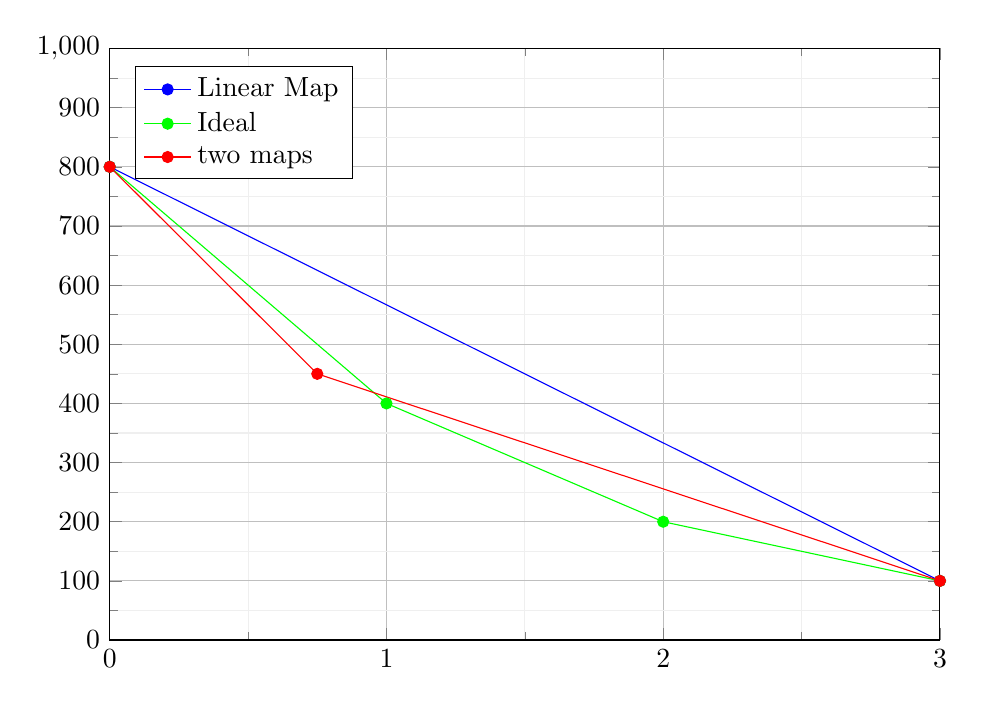
\begin{tikzpicture}
\begin{axis}[
    xmin = 0, xmax = 3,
    ymin = 0, ymax = 1000,
    xtick distance = 1,
    ytick distance = 100,
    grid = both,
    minor tick num = 1,
    major grid style = {lightgray},
    minor grid style = {lightgray!25},
    width = \textwidth,
    height = 0.75\textwidth,
    legend cell align = {left},
    legend pos = north west
]

\addplot[blue, mark = *] 
    coordinates {(0, 800) (3, 100)   };

\addplot[green, mark = *] 
    coordinates { (0, 800) (1, 400) (2, 200) (3, 100)   };

\addplot[red, mark = *] 
    coordinates {(0, 800) (0.75, 450) (3, 100)  };

 

\legend{
    Linear Map, 
    Ideal,
    two maps 
}

\end{axis}

\end{tikzpicture}

\end{document}